\chapter{贝叶斯算法及过滤相关技术}

\section{贝叶斯算法及过滤相关技术}
贝叶斯定理是决策逻辑学的一个分支,使用理论统计学研究概率推论,即根据已经发生的事件来预测将来可能发生的事件。贝叶斯理论假设,如果过去试验中事件的出现的概率己知,那么根据数学方法可以计算出未来试验中事件出现的概率。贝叶斯理论指出,如果事件的结果不确定,那么量化它的唯一方法就是事件的发生概率。
 垃圾邮件过滤其实就是邮件分类问题,把邮件分为垃圾邮件和正常邮件。这就可以应用贝叶斯定理,通过对己经正确分类的邮件来预测新接收的邮件是否为垃圾邮件。
贝叶斯定理的描述如下:
 对于一个统计实验,样本空间s是所有可能结果的集合,并且\begin{math} 
 $\{$B_1,B_2,...B_r$\}$
 \end{math}
是s的一个划分。令$\{$p(A); A S$\}$表示定义在s中所有事件上的一个概率分布,则对于s中的任意事件A和B,有p(A) > 0,P$($ B|A$)$ =P$($B \(\cdot\;\)A$)$/P$($A$)$ 表示条件概率,即在己知A发生的情况下B发生的概率。贝叶斯定理可以表示为:
\begin{equation}
 P(B_i|A) = P(A|B_i)P(B_i)/P(A)  
\end{equation}
其中p$($A$)$ >0,由全概率公式可得
\begin{equation}
 P(A) = P(A|B_j)P(B_j)  
\end{equation}
在公式(2.1)中,p$($Bi|A$)$为后验概率,为似然概率,为先验概率。
\section{朴素贝叶斯的原理}
贝叶斯方法是垃圾邮件过滤中一个重要的方法,该方法的实质是把邮件确定为垃圾邮件或者正常邮件,这是一个分类问题。
设有m个样本空间$\{$C1,C2,...Cn$\}$,邮件d中有n个特征$($W1,W2,...,Wn$)$项,对于给定的类$($k=1,2,…,m$)$,d属于类的概率为
\begin{equation}
 P(C_k|d) = Max\{p(c1|d),p(c2|d),...p(cn|d)\} 
\end{equation}

通过贝叶斯概率公式可得:
\begin{equation}
 P(c_k|d) = \frac{p(d|c_k)p(c_k)}{p(d)}   (k=1,2,...,m)
\end{equation}

其中:
\begin{equation}
 P(d|c_k) = p(w_1,w_2,...,w_n|c_k)
\end{equation}

公式(2.4)中的分母p(d)与类别无关,因而在公式(2.3)中比较最大值的时候可以忽略,所以只需计算概率$p(c_k)$和$p(d|c_k)$即可划分邮件d的类别。

公式(2.4)中,$p(c_k)$为先验概率,很容易计算,但$p(d|c_k)$的计算比较困难,特别是在特征项的数量较大,且特征项之间相依程度较高时,其计算将是极其费时间的。为了简化计算,引入了条件概率独立假设,即假定各特征项之间是相互独立的,这就是朴素贝叶斯过滤器,那么公式(2.5)就可以转换为:
\begin{equation}
 P(d|c_k) = p(w_1,w_2,...,w_n|c_k)=\sum\limits_{i=1}^{n}p(w_i|c_k)
\end{equation}
朴素贝叶斯过滤器的结构如图所示:
\begin{figure}[htbp]
\centering
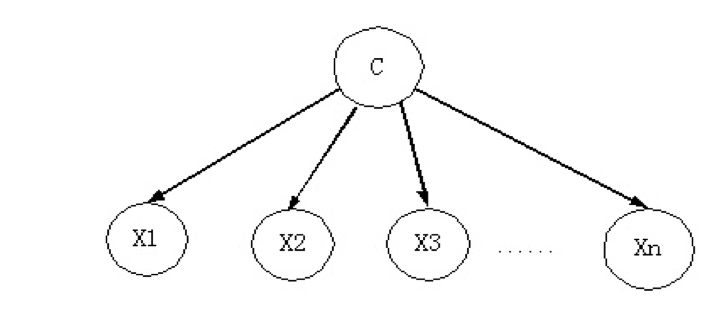
\includegraphics[width=.5\textwidth]{bays1.png}
\caption{朴素贝叶斯过滤器结构图}
\label{fig:logo}
\end{figure}
朴素贝叶斯过滤器主要是利用先验概率求出后验概率,并且根据训练样本集构造过滤器,过滤器根据邮件的后验概率对文本进行分类。
\section{贝叶斯过滤器}
Bogofilter是目前比较流行的贝叶斯过滤器,它的主要原理是朴素贝叶斯理论。Bogofilter建立垃圾邮件和非垃圾邮件贝叶斯概率模型,在贝叶斯原理的实现上,加入了Paul Graham 关于垃圾邮件的过滤理论。该理论大体思想是,在已知的垃圾邮件中,一些单词出现的频率较高,而在合法邮件中,另一些单词出现的频率较高。运用一些众所周知的数学知识,对于每个单词,可以生成一个”垃圾邮件指示性概率”。根据消息中所办含一组词,可以用另一个简单的数学公式来确定文本消息的整体垃圾邮件概率。

Bogofilter将由空格隔开的单词作为特征,并且对特征进行更加严格的定义,譬如,去除单纯包含数字的特征,对于\$20-25这种形式的价格范围,被标记为两个关键词,\$20和\$25等。Bogofilter还使用了平滑技术,来加强过滤器的过滤精度。

 在过滤效率上,Bogofilter采取有效的数据表示,和高效的数据存储技术,获得比较高的过滤效率。Bogofilter使用高性能的Berkerly DB 数据库。Berkerly DB是历史悠久的嵌入式数据库系统,其小巧,可靠,性能高。Berkerly DB 比SQL SERVER 等数据库性能要高10-20倍。
\section{贝叶斯过滤器的优缺点}
朴素贝叶斯算法,其条件概率独立假设,虽然忽略了特征的条件依赖性,但是,在许多实际应用领域中取得了很好的结果,而且其计算简单,降低了算法的复杂性。

 不同与对普通文本的分类,在邮件过滤方面,朴素贝叶斯过滤器也存在一些缺陷。因为邮件分类是一种二类分类问题,且邮件不同于普通文本,有其独特的结构。例如:邮件由邮件头和邮件正文组成,普通的文本分类朴素贝叶斯算法会将邮件头和邮件正文不加区别,而没有考虑到邮件头和邮件正文对邮件类别影响程度的不同。另外邮件分类是一种二类分类问题,两个分类之间是互相影响的,例如合法邮件的误判率低,而非法邮件的误判率高,说明判定一封邮件为非法邮件的阈值过高,为合法邮件的阈值过低。而在普通文本分类时,朴素贝叶斯只是挑选后验概率最大的分类作为文本类别,没有考虑到两类分类中,阈值相关问题。
 
针对朴素贝叶斯在邮件过滤问题上暴露的缺点,我们对朴素贝叶斯过滤器的相关流程做出一系列改进,改进的内容在第四章会有详细描述。
\section{朴素贝叶斯邮件过滤器的扩展}
朴素贝叶斯过滤器在样本学习阶段,通常采用被动学习的方式,这种学习方式没有样本筛选的过程,算法复杂性小,但是这种学习方式造成过滤精度依赖样本的顺序性。

本节提出一种主动学习的贝叶斯过滤器作为普通贝叶斯过滤器的一种扩展。在分类决策阶段。朴素贝叶斯算法是一种基于最小错误率的决策方法,这种决策方法把各种类别的错误判断一视同仁,但是在邮件过滤中,合法邮件误判更应该引起人们重视,所以在此提出最小风险贝叶斯算法,以风险高低作为类别的决策依据,也是在决策阶段对于朴素贝叶斯邮件过滤器的一种扩展。
\subsection{最小风险贝叶斯}
朴素贝叶斯算法是基于最小错误率的决策方法。但是,在邮件的分类与过滤中,合法邮件与垃圾邮件具有不同的特性。合法邮件被判定为垃圾邮件可能给用户带来更大的损失。因此,考虑到各种错误造成的损失不同,可采用最小风险的贝叶斯决策对邮件进行过滤和分类。

基于最小风险的贝叶斯过滤算法是一种特殊的贝叶斯算法,它把邮件分为两类,即合法邮件和非法邮件。最小风险贝叶斯算法是用来增强前面描述的朴素贝叶斯过滤器的性能,降低邮件过滤的风险,以得到一个风险最小的邮件过滤器,是对朴素贝叶斯进行的修正。最小风险贝叶斯的邮件过滤算法,对合法邮件判断为非法邮件以及非法邮件判断为合法邮件定义不同的风险,选择风险最小的决策类别,可以有效降低错误决策造成的损失。
\subsection{主动学习贝叶斯}
根据分类学习对训练样本的处理方式,可将分类模型分成两类:被动分类和主动分类模型。被动分类模型也称”从样本中学习” ,它随机的选择训练样本,被动地接受这些样本的信息,如图2-2。它对于具有严格序关系的训练样本来说是必要的,也是不可改变的。然而绝大部分分类学习中都认为训练样本是独立同分布的,这种被动的学习显示出明显的不足:1)顺序的处理训练样本往往会使学习的过滤器具有顺序相关性,对数据过分敏感;2)遇到噪音样本时,会使这种噪音一直传播下去,影响分类精度3)缺乏综合未带标注样本信息的能力。在学习分类模型中,未带标注的样本往往包含有助于分类的信息。在这种情况下,选择好的未带标注的样本,把它加入到当前的过滤器中是相当重要的。主动分类模型对训练样本的选择是主动的,它选择最有利于过滤器性能的样本来训练过滤器,属于更高层次的,具有潜意识的学习,如图2-3
\begin{figure}[htbp]
\centering
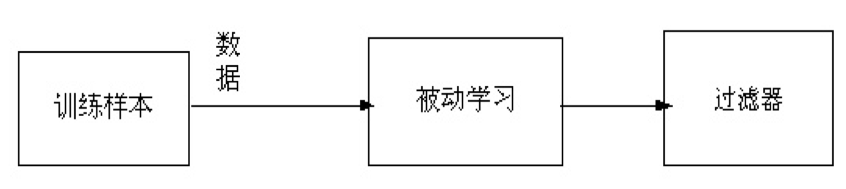
\includegraphics[width=.9\textwidth]{bays2.png}
\caption{被动学习模式}
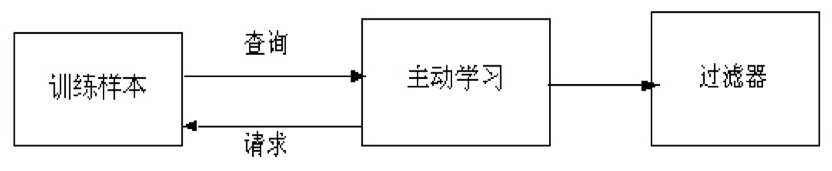
\includegraphics[width=.9\textwidth]{bays3.png}
\caption{主动学习模式}
\label{fig:logo}
\end{figure}

由于贝叶斯网络分类具有增量学习的特性,它更适宜主动学习,在增量地分类和增量学习概率分布方面可以大大的提高效率.传统的学习算法使用给定的训练样本学习分类参数,它所处理的训练样本必须是带有类别标注的,并且一般都假定各训练样本是独立同分布的.相反,主动学习算法在侯选样本集中主动选择测试样本。
\section{邮件评测}
为了能对不同的垃圾邮件过滤算法进行评测,必须有一个可供比较的平台。这包括公共的评测语料,统一的过滤模式和统一的评价方法。
\subsection{邮件过滤语料库}
文本分类问题研究的成功开展,很大程度得益于规范,手工标注类别,公共的文本分类语料库,例如路透社语料,已经成为了标准的测试平台。但是垃圾邮件的语料问题更加复杂,因为邮件涉及到了用户的隐私问题。因此,很多研究者所使用的邮件语料都是私人的,不公开的。这样不同的研究者使用不同的测试语料,所得到的结果就没有很好的可比性,这在一定程度上影响了邮件过滤研究的进展。

垃圾邮件的获得是比较容易的,目前也有很多团队和网站对研究者提供免费下载的垃圾邮件语料,比如SpamArchive.orgAn,nexia.Org等。合法邮件的获得就比较困难,由于邮件使用者往往由于隐私而不愿意公开自己的邮件。所以研究者一般有三种方法获得可以公开的合法邮件语料:

$\blacksquare$ 从新闻组News Group ,邮件列表或者论坛获取文件作为合法邮件。SpamAssassin语料。Ling-Spam语料就是采用这种方法。

$\blacksquare$ 将邮件进行特征选择和向量化处理,公开每个邮件所对应得向量。Spambase就是这种方式。

$\blacksquare$ 将邮件进行编码或者加密,公开的是加密后的邮件。比如PU语料库就是采用这种方式。
本文对算法作进行试验采用了两种邮件集,一个的是全国搜索引擎和网上信息挖掘学术研讨会(SEWM 2008)中文Web信息检索评测中的垃圾邮件过滤评测中,华南理工大学负责收集研制的SEWM 2008邮件集;一个是文本检索会议(text  retrieal conference,简称TREC )提出的trec07p语料库。

SEWM 2008邮件集中的正常邮件来源于三个部分。一个是项目组成员提供的私人邮件;一个是公开邮件群发送的实际邮件;还有按照实际私人邮件和公开邮件的主题、词频、附件等分布特征,通过Internet抓取到邮件内容合成的电子邮件。 其垃圾邮件全部来源于本实验室实际运行邮件服务器上所截获以及用户报告的垃圾邮件,经过部分去重并与其他公开垃圾邮件样本集进行对照后挑选得到。 最后构造的private邮件集中总共包含99054封邮件,其中有24054封正常邮件,75000封垃圾邮件

文本检索会议(text  retrieval conference,简称TREC )从2005年开始构造邮件数据集,其中Trec06数据集加入了中文语料。而Trec07语料总共包括75339封邮件,其中25,220封ham和50119封spam。
\subsection{邮件过滤模式}
邮件过滤模式包括两种,一种是离线过滤模式,一种是在线过滤模式。离线过滤模式是先通过训练邮件集的训练,得到邮件过滤模型,再通过训练得到的邮件模型,对待测试邮件集进行过滤。在线过滤模型运用用户反馈在线更新模型库,然后通过更新的模型判断邮件类别。

 通过对实际的反垃圾邮件应用需求进行抽象,得到的电子邮件在线过滤模式如图6-1所示,以过滤器和学习器为中心分为过滤和学习两部分。过滤器根据在线更新的知识库,过滤按时间顺序输入的邮件流,对每个邮件做出Spam 或Ham 的判断。学习器根据客户反馈对每个邮件的过滤结果进行在线学习,学习的结果进一步精化过滤器的知识库,使得下一个邮件到来时能提高过滤器的性能。
\begin{figure}[htbp]
\centering
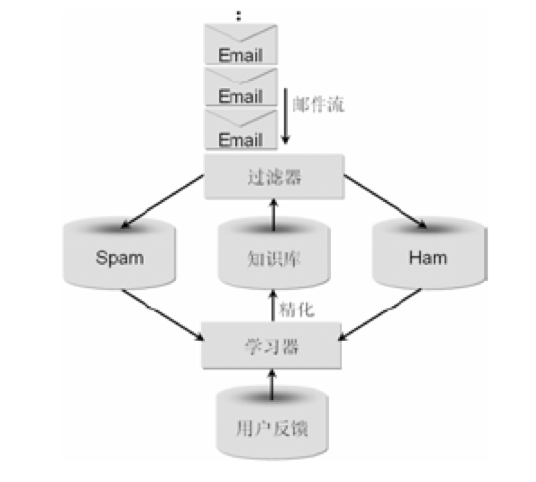
\includegraphics[width=.8\textwidth]{bays4.png}
\caption{电子邮件在线过滤模式}
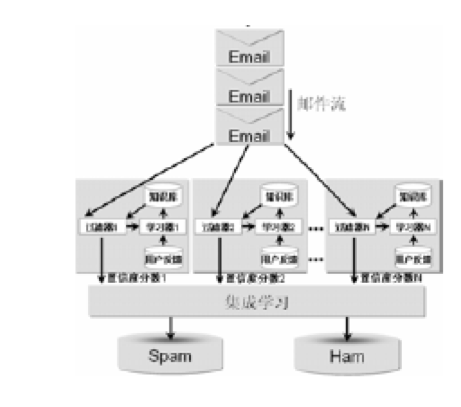
\includegraphics[width=.8\textwidth]{bays5.png}
\caption{离 线 过 滤 模 式}
\label{fig:logo}
\end{figure}
随着过滤器的不断使用和客户不断反馈,学习器逐渐收集了很多带有客户反馈的邮件,每次学习时都可以使用当前收集到的带反馈邮件集进行训练。在TREC Spam 任务中,采用标准答案(Golden Standard)来模拟客户反馈。由于实际应用中客户不一定能够及时正确的给出反馈,所以TREC Spam 任务用立即反馈和延时反馈两种类型来模拟不同的客户反馈时机。立即反馈对于过滤后的每一个邮件能够立刻得到标准答案,通过学习可以马上精化知识库。延时反馈对于过滤后的邮件有可能要过一段时间才能得到答案,甚至永远得不到答案或是得到错误的答案。
\subsection{评价体系}
垃圾邮件过滤的性能评价通常借用文本分类的相关指标。具体地,假设待测试的邮件集合中共有N封邮件,一个垃圾邮件过滤系统的判定结果如下表所示:
\begin{table}[!htbp]
\centering
\begin{tabular}{|c|c|c|}% 通过添加 | 来表示是否需要绘制竖线
\hline  % 在表格最上方绘制横线
&实际为垃圾邮件&实际为合法邮件\\
\hline  %在第一行和第二行之间绘制横线
实际为合法邮件&A&B\\
\hline % 在表格最下方绘制横线
系统判定为合法邮件&C&D\\
\hline % 在表格最下方绘制横线
\end{tabular}
\end{table}

其中,$N=A+B+C+D=N_s+N_h$,其中$N_s=A+C$为实际的垃圾邮件数目,为实际的合法邮件数目。

在评价体系中,本节主要介绍三种评价体系:沿用传统文本分类的评价系统,	ROC 评价方法,以及TREC评测方法。

$\blacksquare$ 沿用传统文本分类的评价系统
定义如下几个评价指标来衡量不同垃圾邮件过滤系统的性能:
(1) 召回率(Recall) :$R=\frac{A}{A+C}=\frac{A}{N}$ ,即垃圾邮件的检出率。这个指标反映了过滤系统发现垃圾邮件的能力,召回率越高,”漏网”的垃圾邮件就越少。

(2)正确率(Precision):$R=\frac{A}{A+B}$ 即垃圾邮件检对率。正确率反应了过滤系统”找对”垃圾邮件的能力,正确率越大,将非垃圾邮件误判为垃圾邮件的数量越少。

(3)精确率(Accuracy):$Accur=\frac{A+D}{N}$ ,即对所有邮件(包括垃圾邮件和合法邮件)的判对率。

(4)错误率(Error rate):$Err=\frac{B+C}{N}=1 Accur$ 即对所有邮件(包括垃圾邮件和合法邮件)的判错率。

(5)F值:$F=\frac{2PR}{R+P}$ F实际上是召回率和正确率的调和平均,它将召回率和正确率综合成一个指标。

除此之外,垃圾邮件过滤中还常常采用虚报率(Fallout)、漏报率(Miss rate)等指标。

另外,我们在前面提到,在实际的垃圾邮件过滤中,人们往往不希望将合法邮件误判成垃圾邮件。为了表示不同情况下垃圾邮件系统的代价。Androutsopoulos等人提出了代价因子CR的概念。设合法邮件误判为垃圾邮件的损失为是垃圾邮件判为合法邮件的入倍。则可以定义:

垃圾邮件系统的加权错误率 $WErr=\frac{B+C}{N_h+N_s}$

在没有任何垃圾邮件过滤器(即所有的垃圾邮件被当成合法邮件)的情况下,可以计算基准的加权错误率: $WErr=\frac{N_s}{N_1+N_s}$

于是,代价因子$TCR=\frac{WErr_b}{WErr}=\frac{N_s}{B+C}$,TCR越高,表明当前垃圾邮件过滤系统的成本越低。

$\blacksquare$ ROC评价方法
在现实问题当中,代价因子CR往往是无法确定的,甚至是变化非常大的。而且合法邮件和垃圾邮件的数目之比N : NS,这个数值也是无法确定并且变化非常大的。而上面所述的评价方法只能评价算法在某一个具体条件下的性能。所以,对垃圾邮件问题来说,必须使用一种能反映各种条件下算法性能的评价方法,ROC就是这样的方法。

在ROC图中,横轴表示ham misclassification rate(hmr),即将合法邮件漏判率,对应于$WErr=\frac{B}{B+D}$;纵轴表示spam misclassification rate(smr),即垃圾邮件漏判率,对应于$WErr=\frac{C}{A+C}$,即1-Recall。。在ROC中,每一个点都对应这样一个(hmr,smr)点。调整问题条件,每个过滤器都会得到一系列这样的点,最后形成一条ROC曲线。如图 3-6中的红色曲线。

在ROC图中的两个点,左上方的点总是比右下方的点更优,因为左上方的点有更小的hmr,和更小的smr。

对于两个算法来说,ROC曲线越靠左上的算法性能越优。对于机器学习算法来说,一般可以通过调整阈值的方法来得到ROC曲线。在垃圾邮件过滤算法中,产生ROC 曲线方法如下:对于一批测试样本中的每封邮件,使用过滤器依次对其进行打分产生一个score值,反映该邮件为spam的可能性。若确定了所有邮件的score值,我们可以通过动态调整阈值t来获得每种可能的hmr%以及对应的smr%,即通过动态调整阈值t,我们可以将smr%表示成hmr%的某个函数,从而画出ROC曲线图
\begin{figure}[htbp]
\centering
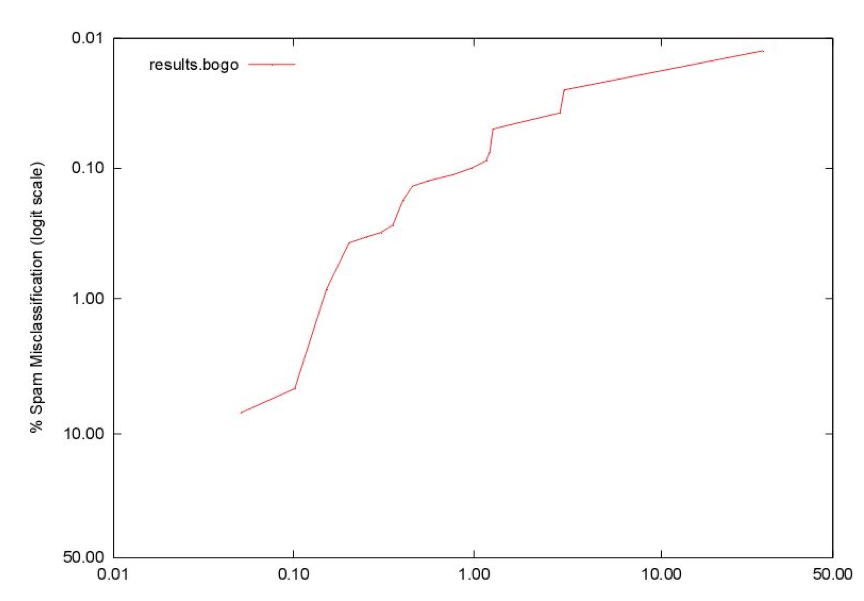
\includegraphics[width=.9\textwidth]{bays6.png}
\caption{ROCA 图}
\label{fig:logo}
\end{figure}

$\blacksquare$ TREC 2005 SPAM track 的评测方法

文本检索会((Text Retrieval Conference, TREC)是目前国际上信息检索领域一年一度的学术交流与系统评测活动,由美国NIST(National Institute of Standards and Technology)、DARPA(Defense  Advanced  Research  Projects  Agency)、DARDA(US Department of Defense Advanced Research and Development Activity)等单位共同主办。TREC在2005年新引入了垃圾邮件过滤器的评测。TREC 2005 SPAM track主要使用了4种评测方式:

$\bullet$ hm\%: 合法邮件漏判率hmr(ham misclassification rate),合法邮件被判成垃圾邮件的比例。

$\bullet$ sm\%:  垃圾邮件漏判率smr(spam misclassification rate),垃圾邮件被判成合法邮件的比例。

$\bullet$ 以hm\%为横坐标,以sm\%为纵坐标,取不同的阈值t时,做ROC曲线

$\bullet$ (1-ROCA)\%: ROC曲线的上方的面积。越小越好,物理意义是过滤器给一个随机的合法邮件的spam打分,等于或大于过滤器给一个随机的垃圾邮件的spam打分的概率。

这四个指标数值越小,表示垃圾邮件过滤系统性能越好。


\section{本章小结}
本章介绍了贝叶斯垃圾邮件过滤算法以及邮件评测的相关内容。第一节到第四节主要是贝叶斯算法的一些介绍。其中详细介绍了贝叶斯定理,以及贝叶斯定理在邮件过滤中的应用:朴素贝叶斯算法。并且通过描述朴素贝叶斯算法的优缺点,引出了最小风险贝叶斯算法和主动学习贝叶斯算法,并且介绍了最小风险贝叶斯算法和主动学习贝叶斯算法的基本原理。第五节到第七节主要介绍了垃圾邮件过滤的几种常用技术以及评价垃圾邮件过滤方法所采用的邮件集和评价体系。垃圾邮件过滤技术从简单的黑白名单技术开始,介绍到本论文所采用的贝叶斯过滤技术。本文采用的邮件集有两种,一种是trec07语料库,一种是sewm2008语料库。在评价体系上,本章主要介绍了TREC 2005 SPAM track 运用的评价标准,重点介绍了ROC评价方法。







